\section{QuickDough Framework}\label{sec:framework}
QuickDough is a development framework for FPGA-accelerated applications. It generates FPGA
accelerators for compute intensive kernels rapidly through the use of a pre-built soft
coarse-grained reconfigurable array (SCGRA) overlay. QuickDough also performs application-specific
customization and generates optimized SCGRA overlay as well as communication infrastructure between
the CPU host and the accelerator automatically, integrating both software and hardware generation in
a unified framework.

\begin{figure}
\centering
\subfloat[Conventional FPGA Accelerator]{
\label{fig:hls-accelerator}
\includegraphics[width=0.47\linewidth]{hls-accelerator}}
%\qquad
\hfill
\subfloat[SCGRA Based FPGA Accelerator]{
\label{fig:scgra-accelerator}
\includegraphics[width=0.47\linewidth]{scgra-accelerator}}
\caption{Hybrid CPU-FPGA Computation System}
\label{fig:FPGA-accelerator}
\end{figure}

\figref{fig:hls-accelerator} shows the design of a typical accelerator system. In such system,
on-chip memory is used to buffer data between the host CPU and the accelerator. A controller is also
presented in hardware to control the operations of the accelerator as well as memory transfers. The
entire design must be reimplemented every time a change is made to the accelerator design, going
through the lengthy low-level hardware implementation tool flow. 
On the other hand, \figref{fig:scgra-accelerator} shows the system generated by QuickDough. While it
features a similar overall design as a typical accelerator system, it utilizes a regular SCGRA
overlay instead of irregular random logic to implement the computation and the overlay can be reused
during the design iterations.  

\begin{figure}
    \center{\includegraphics[width=0.65\linewidth]{framework}}
    \caption{QuickDough: FPGA Accelerator Design Methodology Using SCGRA Overlay. The compute
        intensive part of an application can be compiled to a customized SCGRA overlay based FPGA
    accelerator while the rest can be compiled to host CPU.}
    \label{fig:framework}
\end{figure}

\figref{fig:framework} summarizes the hardware-software compilation flow of QuickDough.
Users begin by specifying the regions for accelerations in the form of compute intensive loops.
Once a loop is identified, it is further compiled to an SCGRA overlay based FPGA
accelerator through SCGRA customization and SCGRA compilation while the rest part of the program is
compiled to the processor through a conventional software compilation.

The SCGRA customization decides the optimized design parameters specifically to a loop kernel for
better performance under given constraints such as resource budget. Because of the softness of the
SCGRA overlay, most architectural parameters may optionally be customized, including the processing
elements' operation, pipeline depth, size of array, as well as on-chip buffer size. Also customized
are routines that controls and transfers data to and from the accelerator. Most importantly, the
customization makes all the hardware design details transparent to the users, which makes the whole system
accessible to high-level designers. The user may choose to perform the customization only when the
loop is changed dramatically and previous customization doesn't fit the updated loop.

Once the overlay design is determined, the SCGRA compilation starts to generates the final FPGA
accelerator bitstream for the specified loop kernel. To begin, the compute kernel loops are
statically analyzed to produce their corresponding data flow graphs (DFGs) with the customized loop
unrolling factor. Then the DFG is scheduled on the overlay with the scheduling result embedded
directly into the SCGRA overlay to create the final FPGA configuration bitstream. This bitstream, in
combination with the software created binary code, forms the final application that will be executed
during run time.



